\chapter{JIT compiler}
\label{chapter:jit-compiler}

\begin{comment}
\begin{multicols}{2}
\noindent

\textbf{Prerequisites}\\
To read this chapter you are supposed to know how a tracing JIT compiler generate a trace including  hotpath detection, recording, trace compilation, abort and blacklisting (see Chapter \ref{}).

\columnbreak
\noindent
\textbf{What you want to learn}\\
After reading this chapter you will learn how LuaJIT implements these techniques when generating a root trace.
\end{multicols}
\end{comment}

\noindent
In this chapter it will be illustrates how LuaJIT performs trace-base just-in-time compilation. We will investigate how the JIT compiler create a trace and all the aspect related to it. 

Traces generation in LuaJIT follows the canonical working principles characteristic of tracing JITs (see Chapter \ref{chapter:background}):
\begin{itemize}
    \item LuaJIT begins executing bytecode instructions with the interpreter (VM).
    \item While executing bytecode instructions, the VM monitors the execution frequency of potential candidates for hotpath headers (hotloops/hotfunctions).
    \item When a hotpath header is identified, LuaJIT starts recording. It executes bytecode with the VM and it records each executed instruction in parallel.
    \item The IR is incrementally generated in SSA (Static Single Assignment) form.
    \item The IR is optimised applying traditional compiler optimisation.
    \item After recording and optimisation, LuaJIT compiles the trace emitting mcode specific to the architecture.
    \item The bytecode is patched with special bytecode instructions (\texttt{J...}) that force the execution of JIT-compiled loops/functions instead of interpreting them.
    \item Any stage of recording, optimisation or compilation might raise an error that would abort the trace creation.
    \item When the same hotcode generate too many times a trace abort, it is blacklisted. LuaJIT will never try to record it again. The bytecode of that hotloop/hotfunction is patched with a special bytecode instruction (\texttt{I...}) that stops hotspot detection and force execution in the interpreter.
\end{itemize}

\section{Hotpaths detection}

The mechanism used by LuaJIT to detect hotpaths is based on Natural Loop First (NLF) and counter base profiling (see Sec. \ref{subsec:identiy-trace-headers} \ref{subsec:hotpath-detection}). Both loops and functions can generate traces, but hotloops are preferred over hotfunctions.

 Trace heads selection is accomplished with a well-defined implementation. Some bytecode instructions are considered as "special" because they are the only ones that can lead to potential hotpath headers (see table \ref{tab:hotpath-headers}).

\begin{table}[H]
    \centering
    \begin{tabular}{|c|c|}
        \hline
        Operation & Description \\
        \hline
        \texttt{FORL} & Numeric 'for' loop\\
        \texttt{LOOP} & Generic loop\\
        \texttt{ITERL} & Iterator 'for' loop\\
        \texttt{ITERN} & Specialized iterator function next() (NYI)\\
        \texttt{FUNCF} & Fixed-arg Lua function\\
        \texttt{FUNCV} & Vararg Lua function\\
        \hline
    \end{tabular}
    \caption{Bytecode instructions for hotpaths detection}
    \label{tab:hotpath-headers}
\end{table}

\noindent
In order to count the invocation frequency of these instructions, LuaJIT uses a relatively small (64 entries) hash table, containing 16-bit integer counters.

\begin{lstlisting}[style=CStyle, caption=\texttt{lj\_dispatch.h}]
typedef uint16_t HotCount;

/* Number of hot counter hash table entries (must be a power of two). */
#define HOTCOUNT_SIZE		64

/* Global state */
typedef struct GG_State {
  ...
  HotCount hotcount[HOTCOUNT_SIZE];	/* Hot counters. */
  ... 
} GG_State;
\end{lstlisting}

\begin{table}[H]
    \centering
    \begin{tabular}{|c|c|}
        \hline
        Index & value \\
        \hline
        \texttt{0} & \texttt{111} \\
        \texttt{1} & \texttt{108} \\ 
        \texttt{2} & \texttt{111} \\
        \texttt{3} & \texttt{51} \\
        \texttt{...} & \texttt{...} \\
        \texttt{63} & \texttt{111} \\
        \hline
    \end{tabular}
    \caption{Example snapshot of an Hotcount Table}
    \label{tab:my_label}
\end{table}

\noindent
Each counter is initialised by default to 111 and it is decremented by 2 when tracing hotloops or by 1 when tracing hotfunctions. This is how LuaJIT gives preference to natural loops.

\begin{lstlisting}[style=CStyle, caption=\texttt{lj\_dispatch.[c,h], lj\_jit.h}]
/* Hotcount decrements. */
#define HOTCOUNT_LOOP		2
#define HOTCOUNT_CALL		1

#define JIT_PARAMDEF(_) \
  _(\007, hotloop,	56)	/* # of iter. to detect a hotloop/call. */ \

/* Initialize hotcount table. */
void lj_dispatch_init_hotcount(global_State *g)
{
  int32_t hotloop = G2J(g)->param[JIT_P_hotloop]; /* extract hotloop value = 56 */
  HotCount start = (HotCount)(hotloop*HOTCOUNT_LOOP - 1); /* start = 111 */
  HotCount *hotcount = G2GG(g)->hotcount;
  uint32_t i;
  for (i = 0; i < HOTCOUNT_SIZE; i++)
    hotcount[i] = start; /* init hotcouters to 111 */
}
\end{lstlisting}

\noindent
Every time a "special" instruction is executed the corresponding counter in the hash table is decremented. When the counter reaches zero, the VM starts recording. 

The hash function used is a  \textit{modulus} 64 operation of the program counter (PC), which is a true pointer in the process memory. The PC contains the virtual memory address of the current bytecode instruction. Thus, when executing a "special" bytecode instruction the VM decrements a counter at the index \texttt{(PC/4)\%64} in the hotcount table. Consecutive bytecode instructions are stored at consecutive memory location with a step of 4 bytes. For 32 bits architecture the PC has a shape such as \texttt{0x419628d0}, while for 64 bits architecture it is \texttt{0x7fd7493e56dc}.

\begin{figure}[H]
    \centering
	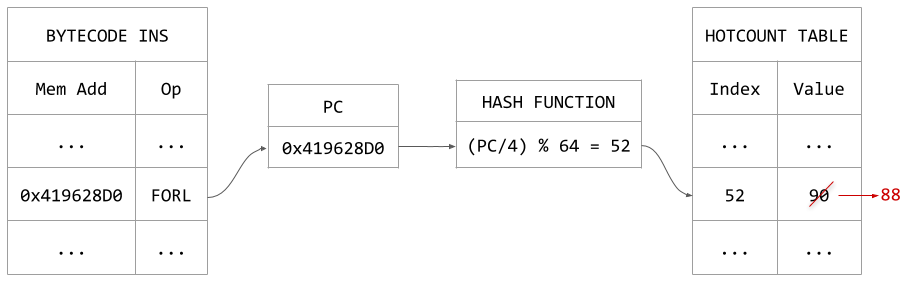
\includegraphics[width=\textwidth]{images/chapter7/HotpathDetection.png}
    \caption{Hotcount decrement for loops}
    \label{fig:hotcount}
\end{figure}

\noindent
Indeed, to set and get hotcount values the following macros are defined.

\begin{lstlisting}[style=CStyle, caption=\texttt{lj\_dispatch.h}]
#define hotcount_get(gg, pc) \
  (gg)->hotcount[(u32ptr(pc)>>2) & (HOTCOUNT_SIZE-1)] /* hotcount[(PC/4)%64] */
#define hotcount_set(gg, pc, val) \
  (hotcount_get((gg), (pc)) = (HotCount)(val))
\end{lstlisting}

\subsection{Architecture specific implementation}

The hotpath detection technique just explained is fully implemented in assembly (in the \texttt{vm\_ARCH.dasc} architecture specific files). 

To give an example, \texttt{vm\_x86.dasc} contains a macro (\texttt{hotloop}) that is executed when a "special" loop instruction occurs (i.e. \texttt{FORL}). In \texttt{hotloop}, the counter is decremented by 2 and, when it reaches zero, the execution flow jumps to \texttt{->vm\_hotloop}. Finally, the VM calls an external C function \texttt{lj\_trace\_hot} (defined in \texttt{lj\_trace.c}) where the counter is reset to 112 and LuaJIT starts recording.

%Entry table 64 entries of 2 bytes each (so 128 total bytes reserved). We suppose that 2 consecutive instructions can collide because there will never be 2 consecutive instruction with a hot counter.
\begin{lstlisting}[style=DynASMStyle, caption=\texttt{vm\_x86.dasc}]
/* Generate the code for a single instruction. */
static void build_ins(...) {
  ...
  switch (op) {
    ...
    case BC_FORL:
    |.if JIT
    |  hotloop RB
    |.endif
    break;
    ... 
  }
}

|// Decrement hashed hotcount and trigger trace recorder if zero.
|.macro hotloop, reg
|  mov reg, PC
|  shr reg, 1
|  and reg, HOTCOUNT_PCMASK
|  sub word [DISPATCH+reg+GG_DISP2HOT], HOTCOUNT_LOOP
|  jb ->vm_hotloop
|.endmacro

|// hotloop counter underflow.
|->vm_hotloop:			
|.if JIT
|  ...
|  call extern lj_trace_hot@8 // (jit_State *J, const BCIns *pc)
|  jmp <3
|.endif

\end{lstlisting}

% code macros dispatch.h
\begin{comment}
\begin{lstlisting}[style=CStyle, caption=\texttt{dispatch.h}]
/* Type of hot counter. Must match the code in the assembler VM. */
/* 16 bits are sufficient. Only 0.0015% overhead with maximum slot penalty. */
typedef uint16_t HotCount;

/* Number of hot counter hash table entries (must be a power of two). */
#define HOTCOUNT_SIZE		64
#define HOTCOUNT_PCMASK		((HOTCOUNT_SIZE-1)*sizeof(HotCount))

/* Hotcount decrements. */
#define HOTCOUNT_LOOP		2
#define HOTCOUNT_CALL		1

/* This solves a circular dependency problem -- bump as needed. Sigh. */
#define GG_NUM_ASMFF	62

#define GG_LEN_DDISP	(BC__MAX + GG_NUM_ASMFF)
#define GG_LEN_SDISP	BC_FUNCF
#define GG_LEN_DISP	(GG_LEN_DDISP + GG_LEN_SDISP)

/* Global state, main thread and extra fields are allocated together. */
typedef struct GG_State {
  lua_State L;				/* Main thread. */
  global_State g;			/* Global state. */
#if LJ_TARGET_MIPS
  ASMFunction got[LJ_GOT__MAX];		/* Global offset table. */
#endif
#if LJ_HASJIT
  jit_State J;				/* JIT state. */
  HotCount hotcount[HOTCOUNT_SIZE];	/* Hot counters. */
#endif
  ASMFunction dispatch[GG_LEN_DISP];	/* Instruction dispatch tables. */
  BCIns bcff[GG_NUM_ASMFF];		/* Bytecode for ASM fast functions. */
} GG_State;

#define GG_OFS(field)	((int)offsetof(GG_State, field))
#define G2GG(gl)	((GG_State *)((char *)(gl) - GG_OFS(g)))
#define J2GG(j)		((GG_State *)((char *)(j) - GG_OFS(J)))
#define L2GG(L)		(G2GG(G(L)))
#define J2G(J)		(&J2GG(J)->g)
#define G2J(gl)		(&G2GG(gl)->J)
#define L2J(L)		(&L2GG(L)->J)
#define GG_G2DISP	(GG_OFS(dispatch) - GG_OFS(g))
#define GG_DISP2G	(GG_OFS(g) - GG_OFS(dispatch))
#define GG_DISP2J	(GG_OFS(J) - GG_OFS(dispatch))
#define GG_DISP2HOT	(GG_OFS(hotcount) - GG_OFS(dispatch))
#define GG_DISP2STATIC	(GG_LEN_DDISP*(int)sizeof(ASMFunction))

#define hotcount_get(gg, pc) \
  (gg)->hotcount[(u32ptr(pc)>>2) & (HOTCOUNT_SIZE-1)]
#define hotcount_set(gg, pc, val) \
  (hotcount_get((gg), (pc)) = (HotCount)(val))
\end{lstlisting}
\end{comment}

\noindent
The same logic is applied for hotfunctions. If a "special" function call instruction is executed the VM decrements a counter by 1 in the hotcount table (using the macro \texttt{hot\_call}). When the counter reaches zero the execution flow jumps to \texttt{->vm\_hotcall}. In this case the VM calls an external C function \texttt{lj\_dispatch\_call} defined in \texttt{lj\_dispatch.c}.

The example above refers to x86 architectures, but similar procedures are used for the other architectures.

\subsection{Hotcount collisions}

The hash function selected  and the use of a relatively small hotcount table lead inevitably to collisions. When the hash function gives the same result, different "special" bytecode instructions (and therefore different potential hotpaths) correspond to the same counter.

In tracing JITs, as mention by Gal et al. \cite{gal2006hotpathvm}, collisions are intentionally tolerated as their impact on the code is relatively limited. Collisions can lead to overestimation of the "hotness" of a code region, triggering "cold" code recording. Thus, false positive may occur. This overestimation may cause slight performance degradation as the compilation cost could be more expensive than simple interpretation of the code. However this degradation can be neglected when analysing the overall performances, especially for very fast JITs such as LuaJIT.

\subsection{Memory address randomisation}
The mechanism used to manage hot counters depends on the memory address where bytecode instructions are located. This technique was adopted because each counter must be attached to the code fragment from where a hotpath is generated. However, this method implies some difficulties in studying the JIT behaviour when the operating systems support Address Space Layout Randomisation (ASLR). ASLR is a memory-protection system that guards against buffer-overflow attacks by randomising the location where executables are loaded into memory by the operating system. Two consecutive runs of the exact same code will generate different memory address for the same bytecode instruction. Code fragments could be attached to different counters of the Hotcount table and the behaviour of the JIT can be different from run to run.

Most operating systems nowadays support ASLR, but this should not be seen as a problem for LuaJIT. Even if code fragments are attached to different counters in the Hotcount table from run to run, LuaJIT tries to guarantee on average relatively similar performance on the whole application. However, in some cases there are peaks of substantial slowness in execution.

ASLR brought significant difficulties in the context of this research while studying LuaJIT. In fact, the approach adopted to overcome this problem was to disable ASLR when examining LuaJIT internals. In this way the JIT behaviour will be deterministic and bytecode instructions will be stored in the same memory addresses from run to run.

\section{Recording}
Once an hotpath has been triggered LuaJIT starts recording. From the hotpath header, bytecode instructions will be recorded while they are executed. Recording continues until either an end-of-trace condition is encountered or the trace is aborted. The control flow is flattened, therefore only taken branches are recorded and functions are generally inlined.

\subsection{Trace compiler state machine}
\label{trace-compiler-states}
The trace compiler (implemented in \texttt{lj\_trace.c}) manages the recording phases. Its behaviour changes according to its current state (possible states are shown in Tab. \ref{tab:trace-compiler-states}). Each state can be either \textit{active} if the \textit{activation bit} is set to 1 (\texttt{0x1\textit{n}}) or \textit{not Active} if the activation bit is set to 0 (\texttt{0x0\textit{n}}). When an error occurs the trace compiler changes its current state to \textit{not active} before switching to state \texttt{LJ\_TRACE\_ERR} and abort.


\begin{lstlisting}[style=CStyle, caption=\texttt{lj\_jit.h}]
/* Trace compiler state. */
typedef enum {
  LJ_TRACE_IDLE, /* Trace compiler idle */
  LJ_TRACE_ACTIVE = 0x10,
  LJ_TRACE_RECORD, /* BC recording active */
  LJ_TRACE_START, /* New trace started */
  LJ_TRACE_END, /* End of trace. */
  LJ_TRACE_ASM, /* Assemble trace */
  LJ_TRACE_ERR /* Trace aborted with error */
} TraceState;
\end{lstlisting}

\begin{table}[H]
    \centering
    \begin{tabular}{|c|c|c|}
         \hline
         Trace compiler state & Active & Not Active\\
         \hline
         \texttt{LJ\_TRACE\_IDLE} & \texttt{0x00} & \texttt{0x00}\\
         \texttt{LJ\_TRACE\_ACTIVE} & \texttt{0x10} & \texttt{0x00}\\
         \texttt{LJ\_TRACE\_RECORD} & \texttt{0x11} & \texttt{0x01}\\
         \texttt{LJ\_TRACE\_START} & \texttt{0x12} & \texttt{0x02}\\
         \texttt{LJ\_TRACE\_END} & \texttt{0x13} & \texttt{0x03}\\
         \texttt{LJ\_TRACE\_ASM} & \texttt{0x14} & \texttt{0x04}\\
         \texttt{LJ\_TRACE\_ERR} & \texttt{0x15} & \texttt{0x05}\\
         \hline
    \end{tabular}
    \caption{Trace compiler state encoding}
    \label{tab:trace-compiler-states}
\end{table}

\noindent
The trace compiler behaviour is coordinated by a finite state machine (Fig. \ref{fig:trace-state-machine}) implemented in the function \texttt{trace\_state} at \texttt{lj\_trace.c}.
 
\begin{figure}[H]
\begin{tikzpicture}[->,>=stealth',shorten >=1pt,auto,node distance=2.8cm, semithick]
  \tikzstyle{every state}=[fill=none,draw=black,text=black]

  \node[state] (IDLE)   {IDLE};
  \node[state]  (START) [right=2 cm of IDLE] {START};
  \node[state]  (RECORD) [right=2 cm of START] {RECORD};
  \node[state]  (END) [right of=RECORD] {END};
  \node[state]  (ASM) [right of=END] {ASM};
  \node[state]  (ERR) [below of=RECORD] {ERR};
    
  \path (IDLE)      edge node {new trace} (START)
        (START)     edge node {start rec} (RECORD)
        (RECORD)    edge node {stop rec} (END)
        (RECORD)   edge node {abort} (ERR)
        (END)       edge node {assemble} (ASM)
        (RECORD)    [loop above] edge node [shift={(1.4,-0.6)}] {rec next ins} (RECORD)
        (ASM)   [bend right] edge node  {trace successfully compiled} (IDLE)
        (ERR)   [bend left] edge node [shift={(-0.7,-0.7)}] {error detected} (IDLE)
        (END)   [bend left] edge node  [shift={(0.5,-0.5)}] {abort} (ERR)
        (ASM)   [bend left] edge node  [shift={(0.5,-0.5)}] {abort} (ERR);
\end{tikzpicture}
\caption{Trace compiler state machine}
\label{fig:trace-state-machine}
\end{figure}

\begin{multicols}{2}
\begin{lstlisting}[style=CStyle, caption=\texttt{lj\_trace.c}]
/* State machine for the trace compiler*/
static TValue *trace_state(...) {
  do {
  retry:
    switch (J->state) {
    case LJ_TRACE_START:
      J->state = LJ_TRACE_RECORD;
      @@trace_start(J)@@;
      lj_dispatch_update(J2G(J));
      break;

    case LJ_TRACE_RECORD:
      setvmstate(J2G(J), RECORD);
      lj_vmevent_send_(L, RECORD, ...)
      @@lj_record_ins(J)@@;
      break;

    case LJ_TRACE_END:
      setvmstate(J2G(J), OPT);
      /* Perform optimisations */
      @@lj_opt_dce(J);@@
      /* Loop optimisation failed? */
      if (@@lj_opt_loop(J)@@) { 
	      ...
	      /* Try to continue recording*/
	      J->state = LJ_TRACE_RECORD;  
	      break;
	    }
      @@lj_opt_split(J)@@;
      @@lj_opt_sink(J)@@;
      J->state = LJ_TRACE_ASM;
      break;

    case LJ_TRACE_ASM:
      setvmstate(J2G(J), ASM);
      @@lj_asm_trace(J, &J->cur)@@;
      @@trace_stop(J)@@;
      setvmstate(J2G(J), INTERP);
      J->state = LJ_TRACE_IDLE;
      lj_dispatch_update(J2G(J));
      return NULL;

    default:  
      /* Trace aborted asynchronously*/
      setintV(L->top++, LJ_TRERR_RECERR);
      /* fallthrough */
      
    case LJ_TRACE_ERR:
      if (trace_abort(J)) {
        goto retry;
      }
      setvmstate(J2G(J), INTERP);
      J->state = LJ_TRACE_IDLE;
      lj_dispatch_update(J2G(J));
      return NULL;
    }
    
  } while (J->state > LJ_TRACE_RECORD);
  return NULL;
}
\end{lstlisting}
\end{multicols}

\noindent
The following paragraphs describe in details each of these states.

\subsection{Start recording}
As mentioned in the previous paragraph, when a hotloop is detected the VM calls an external C function \texttt{lj\_trace\_hot}. For hotfunctions the VM calls \texttt{lj\_dispatch\_call}, but the execution flow also goes to \texttt{lj\_trace\_hot} after some initialisations. Thus, \texttt{lj\_trace\_hot} can be considered as the starting point for trace recording. In this function the counter is reset to 112, the state is changed to \texttt{LJ\_TRACE\_START} and the execution flows goes to \texttt{lj\_trace\_ins}, which begins the trace compiler state machine previously described.

\begin{figure}[H]
    \centering
	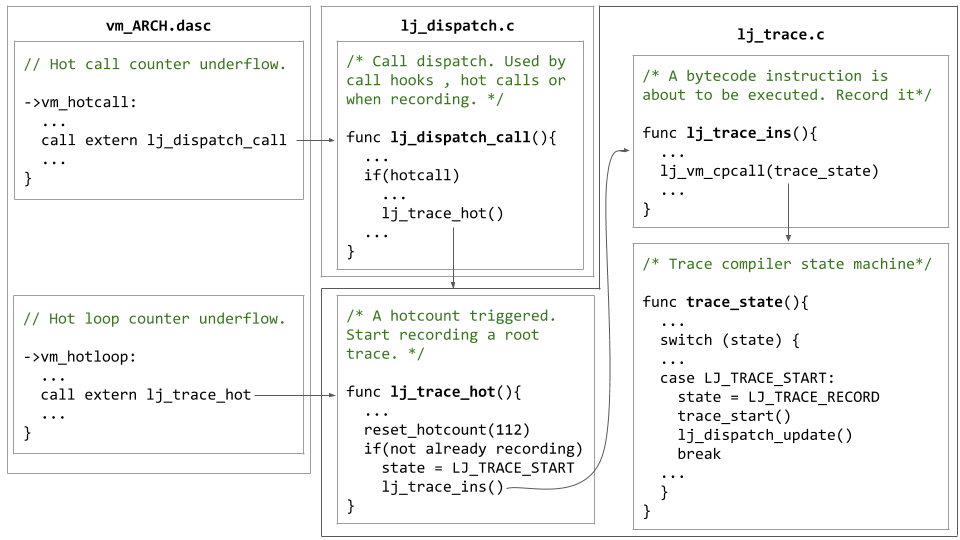
\includegraphics[width=\textwidth]{images/chapter7/start_recording.png}
    \caption{Start recording}
    \label{fig:start-recording}
\end{figure}

\noindent
When the state is \texttt{LJ\_TRACE\_START} the following actions are performed: (i) the trace compiler state is changed to \texttt{LJ\_TRACE\_RECORD}; (ii) the function \texttt{trace\_start} performs initial setup to start a new trace; (iii) the function \texttt{lj\_dispatch\_update} prepares the dispatcher, so that each bytecode instructions executed by the VM will be henceforward recorded.

\subsection{Recording}
Recording will be done executing in an infinite loop \texttt{lj\_dispatch\_ins} and \texttt{lj\_trace\_ins} until recording stops or an error occurs. The trace compiler state is \texttt{LJ\_TRACE\_RECORD} and for each instruction the execution flow goes to \texttt{lj\_record\_ins} (defined in \texttt{lj\_record.c}). This function is responsible for recording a bytecode instruction before it is executed. It contains a huge switch case on all possible bytecodes. Finally, from each bytecode instruction, LuaJIT emits the corresponding IR instruction. Therefore, the IR is incrementally generated.

\begin{figure}[H]
    \centering
	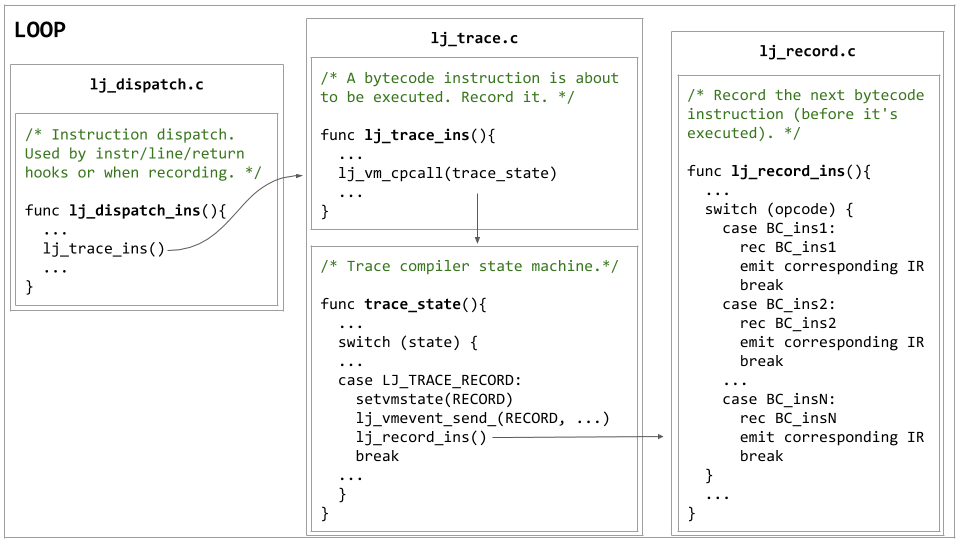
\includegraphics[width=\textwidth]{images/chapter7/Record_loop.png}
    \caption{Recording a bytecode instruction}
    \label{fig:recording-bytecode}
\end{figure}

\noindent
If no error occurs, the loop is iterated \textit{n} times, where \textit{n} is the number of bytecode instructions of the hotpath.

When the trace compiler records the last bytecode instruction of the hotcode (e.g. \texttt{FORL}), the function \texttt{lj\_record\_stop} is executed. It stops recording and sets the trace compiler state to \texttt{LJ\_TRACE\_END}.

\subsection{Ending recording}
Once the recording is concluded, LuaJIT applies optimisations on the IR in SSA form: dead code elimination, loop optimisation, split pass and sink optimisation. It should be noted that most optimisations are performed on-the-fly once all the IR in SSA form is emitted. Hence, eliminated IR instructions are either simply not emitted or ignored during mcode generation \cite{luajit-wiki}. Finally, the trace compiler state is changed to \texttt{LJ\_TRACE\_ASM}.

% **** Optimisations ****
\section{Optimisation}

It is possible to distinguish between three types of optimisation in the code.
First of all, the optimisations of the optimisation engine.
They are implemented in the \texttt{lj\_opt\_*.c} files, hence they can be easily identified.
These optimisations are can be either: (i) global optimisations, which are run on the
entire IR once at the end of the recording phase, during the
\emph{LJ\_TRACE\_END} state (see \ref{Subsec:opt-dce}, \ref{Subsec:opt-loop},
\ref{Subsec:opt-split}, \ref{Subsec:opt-sinking}) or (ii) local optimisations,
which are applied while recording a trace (see \ref{Subsec:narrowing},
\ref{Subsubsec:fold}, \ref{Subsubsec:mao}). Finally, there is a plethora of
optimisations and heuristics applied in various parts of the code (ssee LuaJIT wiki on
optimisation \cite{luajit-opt}).

% Dead code elimination
\subsection{Dead code elimination}
\label{Subsec:opt-dce}

Dead Code Elimination (DCE) is performed by the \textit{lj\_opt\_dce main} function
in two phases. During the first phase, which is called "mark snap", it marks all IR
instructions that are referenced by a snapshot. In the second phases, which is called
"propagate", it iteratively marks all IR instruction that are referenced by an already
marked IR instruction while replacing non-marked IR instruction by nops.

% Loop optimisations
\subsection{Loop optimisations}
\label{Subsec:opt-loop}

Loop optimisation is a way to improve code hoisting for traces based on
loops. In fact, LuaJIT should try to hoist most invariant instruction and guards
in such a way that traces that do not match the current dynamic profile of
the code (assumptions on data or type) are exited as soon as possible.
Unfortunately, due to the dynamic nature of the IR generated, a trace contains many
guards which are control-dependent, making little room for loop-invariant
code motion (LICM). The solution used here is a copy-substitution of the body
of the loop. It basically consists in always unrolling the loop once before the
actual loop instruction. This allows the code executed inside the loop to
contains only variant instructions.

% Split optimisations
\subsection{Split optimisations}
\label{Subsec:opt-split}

The split optimisation is only used by 32-bits architecture and splits the
64-bits IR instructions into multiple 32-bits once.

% Sinking optimisations
\subsection{Sinking optimisations}
\label{Subsec:opt-sinking}
This is a very useful optimisation that allows to avoid many temporaries and
unnecessary memory accesses and allocations by keeping the values of interest
directly in register. Since memory modifications are not performed, we need a way
to remember the writes in case those value escape the execution path
(they are not temporary anymore). For this purpose snapshots are used (see Section \ref{sec:snapshots}).
This optimisation is implemented in \texttt{}{lj\_opt\_sink.c}.and a detailed
explanation of it is available on the wiki \cite{luajit-sink}.

% Narrowing optimisations
\subsection{Narrowing optimisations}
\label{Subsec:narrowing}

LuaJIT performs the narrowing of Lua numbers (double) into integers when it seems
to be useful. It uses demand-driven (by the backend) narrowing for index
expressions, integer arguments (FFI), bit operations and predictive
narrowing for induction variables. It emits overflow check instruction when
necessary. Most arithmetic operations are never narrowed. More details are illustrated in the comment section of \texttt{lj\_opt\_narrow.c}.

% Fold engine
\subsection{Fold engine}
\label{Subsec:fold}

The fold engine implement a rule-based mechanism. Rules are declared using the
\textit{LJFOLD} macro which contains the IR opcode and a rule on the parameters it
applies. During the LuaJIT buildvm (more precisely the \texttt{buildvm\_fold.c}
file), these rules are scanned and the \texttt{lj\_foldef.h} file is generated.
It contains a semi-perfect hash table for constant-time rule lookups, where each
entry respect the format depicted in Table \ref{tab:fold-format}. It also
contains a second table with the function to call if a corresponding rule
matches.

\begin{table}[H]
\centering
\caption{Fold hash table, bit pattern entry}
\label{tab:fold-format}
\begin{tabular}{|c|c|c|c|c|}
\hline
8 bits           & 7 bits            & 7 bits            & 2 bits   & 8 bits                      \\ \hline
index fold table & fold instr opcode & left instr opcode & 00       & right instr opcode      \\ \hline
index fold table & fold instr opcode & left instr opcode & \multicolumn{2}{c|}{literal field} \\ \hline
\end{tabular}
\end{table}

\subsubsection{Fold optimisations}
\label{Subsubsec:fold}

The fold optimisations preformed by the FOLD engine are implemented in the
\texttt{lj\_opt\_fold.c} file. They can be classified in five well-known techniques: (i) constant folding, (ii) algebraic simplifications, (iii) re-association, (iv) common sub-expression
elimination, and (v) array bounds check elimination.

\subsubsection{Memory access optimisations}
\label{Subsubsec:mao}

The memory access optimisation perform by the FOLD engine and implemented
in \texttt{lj\_opt\_mem.c}. It consists of three components: (i) the alias
analysis using high-level semantic disambiguation, (ii) load to load and store to load
forwarding, and (iii) finally dead-store elimination.



\section{Assemble trace}
When the compiler state machine reaches the state \texttt{LJ\_TRACE\_ASM}, the trace is assembled. The main function responsible for this task is \texttt{lj\_asm\_trace} (defined in \texttt{lj\_asm.c}). 
Each IR instruction previously generated is assembled through the function \texttt{asm\_ir} that contains a huge switch case on all possible IR codes. 

The implementation of the assembler is divided in three different files: (i) \texttt{lj\_asm.c} contains the platform-independent code, (ii) \texttt{lj\_asm\_ARCH.h} contains the architecture dependent code (e.g. x86), and (iii) \texttt{lj\_emit\_ARCH.h} contains the helper functions to generate instructions for a specific instruction-set. An IR instruction can be translated into $M\geq1$ machine code instructions.

\begin{figure}[H]
    \centering
	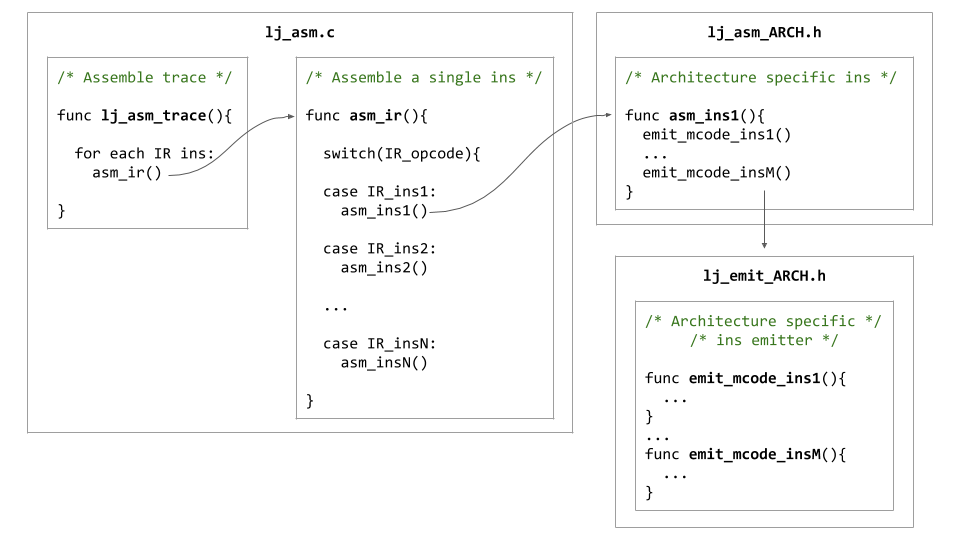
\includegraphics[width=\textwidth]{images/chapter7/Assemble_Trace.png}
    \caption{Assemble trace}
    \label{fig:assemble-trace}
\end{figure}

\noindent
At the end of the assemble phase the hotpath header bytecode is patched with the adequate \texttt{J...} operation. This will force the VM to execute the JIT-compiled trace, instead of interpreting the corresponding bytecode instructions. When the execution of the trace will be completed, the control flow goes back to the VM that restart interpreting the bytecode instructions after the hotcode.

The function \texttt{trace\_stop} is responsible to stop tracing and to patch the bytecode (see Tab. \ref{tab:jitcompiled-operations}).

\begin{figure}[H]
    \centering
	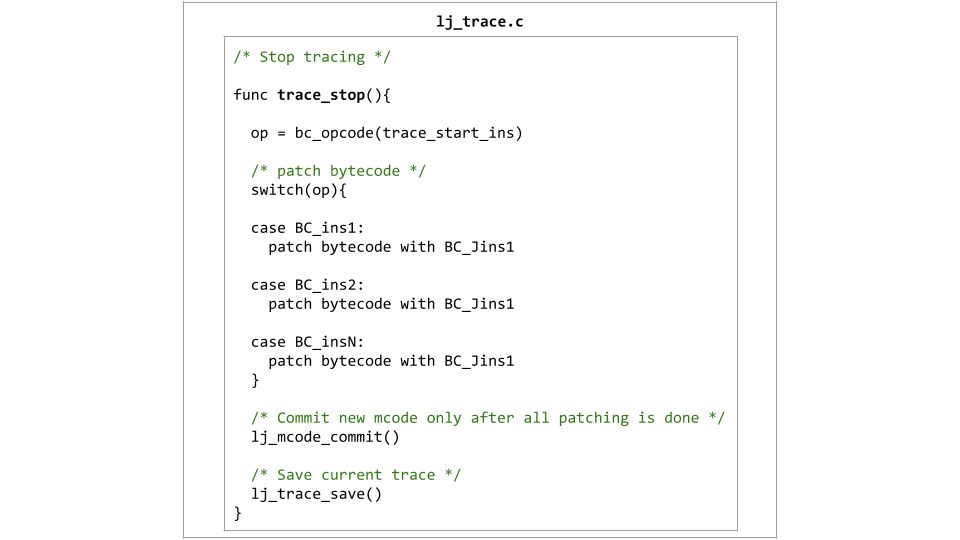
\includegraphics[width=\textwidth]{images/chapter7/Trace_Stop.png}
    \caption{Stop tracing}
    \label{fig:stop-tracing}
\end{figure}

\begin{table}[H]
    \centering
    \begin{tabular}{|c|c|c|}
        \hline
        'Standard' op & JIT-compiled op & Description \\
        \hline
        \texttt{FORI} & \texttt{JFORI} & Numeric 'for' loop init\\
        \texttt{FORL} & \texttt{JFORL} & Numeric 'for' loop\\
        \texttt{LOOP} &  \texttt{JLOOP} & Generic loop\\
        \texttt{ITERL} & \texttt{JITERL} & Iterator 'for' loop\\
        \texttt{FUNCF} & \texttt{JFUNCF} & Fixed-arg Lua function\\
        \texttt{FUNCV} & \texttt{JFUNCV} & Vararg Lua function\\
        \hline
    \end{tabular}
    \caption{Bytecode instructions to force JIT-compiled trace execution}
    \label{tab:jitcompiled-operations}
\end{table}

\section{Trace Abort}
\subsection{Abort}
An abort can occur at any stage of the just-in-time compilation: recording, optimisation or assembling.  Tab. \ref{tab:abort-messages} collects all possible causes of abort.

\begin{center}
\begin{longtable}{|c|c|c|}
\hline
\textbf{Err Num} & \textbf{Err Code} & \textbf{Description}\\
\hline
\multicolumn{3}{|c|}{\texttt{/* Recording */}}  \\
\hline
0 & \texttt{RECERR} &	error thrown or hook called during recording\\
1 & \texttt{TRACEUV} &	trace too short\\
2 & \texttt{TRACEOV} &	trace too long\\
3 & \texttt{STACKOV} &	trace too deep\\
4 & \texttt{SNAPOV} &	too many snapshots\\
5 & \texttt{BLACKL} &	blacklisted\\
6 & \texttt{RETRY} &   retry recording\\
7 & \texttt{NYIBC} &   NYI: bytecode \texttt{\%d}\\
\hline
\multicolumn{3}{|c|}{\texttt{/* Recording loop ops */}}  \\
\hline
8 & \texttt{LLEAVE} & leaving loop in root trace\\
9 & \texttt{LINNER} &	inner loop in root trace\\
10 & \texttt{LUNROLL} &	loop unroll limit reached\\
\hline
\multicolumn{3}{|c|}{\texttt{/* Recording calls/returns */}}   \\
\hline
11 & \texttt{BADTYPE} &	bad argument type\\
12 & \texttt{CJITOFF} &	JIT compilation disabled for function\\
13 & \texttt{CUNROLL} &	call unroll limit reached\\
14 & \texttt{DOWNREC} &	down-recursion, restarting\\
15 & \texttt{NYIFFU} &	NYI: unsupported variant of FastFunc \texttt{\%s}\\
16 & \texttt{NYIRETL} &	NYI: return to lower frame\\
\hline
\multicolumn{3}{|c|}{\texttt{/* Recording indexed load/store */}}   \\
\hline
17 & \texttt{STORENN} &	store with nil or NaN key\\
18 & \texttt{NOMM} &	missing metamethod\\
19 & \texttt{IDXLOOP} &	looping index lookup\\
20 & \texttt{NYITMIX} &	NYI: mixed sparse/dense table\\
\hline
\multicolumn{3}{|c|}{\texttt{/* Recording C data operations */}}   \\
\hline
21 & \texttt{NOCACHE} &	symbol not in cache\\
22 & \texttt{NYICONV} &	NYI: unsupported C type conversion\\
23 & \texttt{NYICALL} &	NYI: unsupported C function type\\
\hline
\multicolumn{3}{|c|}{\texttt{/* Optimisations */}}   \\
\hline
24 & \texttt{GFAIL} &	guard would always fail\\
25 & \texttt{PHIOV} &	too many PHIs\\
26 & \texttt{TYPEINS}     &	persistent type instability\\
\hline
\multicolumn{3}{|c|}{\texttt{/* Assembler */}}   \\
\hline
27 & \texttt{MCODEAL} &	failed to allocate mcode memory\\
28 & \texttt{MCODEOV} &	machine code too long\\
29 & \texttt{MCODELM} &	hit mcode limit (retrying)\\
30 & \texttt{SPILLOV} &	too many spill slots\\
31 & \texttt{BADRA} &	inconsistent register allocation\\
32 & \texttt{NYIIR} &	NYI: cannot assemble IR instruction \texttt{\%d}\\
33 & \texttt{NYIPHI} &	NYI: PHI shuffling too complex\\
34 & \texttt{NYICOAL} &	NYI: register coalescing too complex\\
\hline
\caption{Trace compiler error messages}
\label{tab:abort-messages}
\end{longtable}
\end{center}
\noindent
An \textit{asynchronous} trace abort is detected by the trace compiler state machine when the current state does not match any of the possible \textit{active} states. The execution flow ends up in the \texttt{default} event of the switch case and recoding aborts.

On the other hand, when a trace aborts \textit{synchronously} the function \texttt{lj\_trace\_err} is called. This throws an error and the current state is set to \textit{not active}. In \texttt{lj\_trace\_ins} the function call of \texttt{trace\_state} through \texttt{lj\_vm\_cpcall} will return zero, thus the trace compiler state changes to \texttt{LJ\_TRACE\_ERR}. In this case the trace will abort and, if it is a root trace, the PC of the starting bytecode instruction is penalised (penalisation and blacklisting are explained in the following section).

The functions called to throw an error and to abort are shown respectively in Fig. \ref{fig:throw-err} and Fig. \ref{fig:abort-mechanism}

For some abort causes it is quite intuitive to catch what they are supposed to mean (e.g. error thrown, trace too short, long or deep, too many snapshots). For others, it can be more tricky to get their real meaning. Error 5 (blacklisted) means that while recording a trace, the interpreter hits a  blacklisted bytecode instruction. In this case recording aborts and the execution goes back to the interpreter. LuaJIT does not allow to retry compilation of blacklisted code fragments in a different context. NYI errors mean Not-Yet-Implemented features of the tracing JIT. All aspects of Lua are implemented in LuaJIT's interpreter, but not all of them are implemented in LuaJIT's JIT compiler. When recording encounters a bytecode instruction which is not-yet-implemented in its corresponding JIT version, trace creation is aborted. 

\begin{figure}[H]
    \centering
	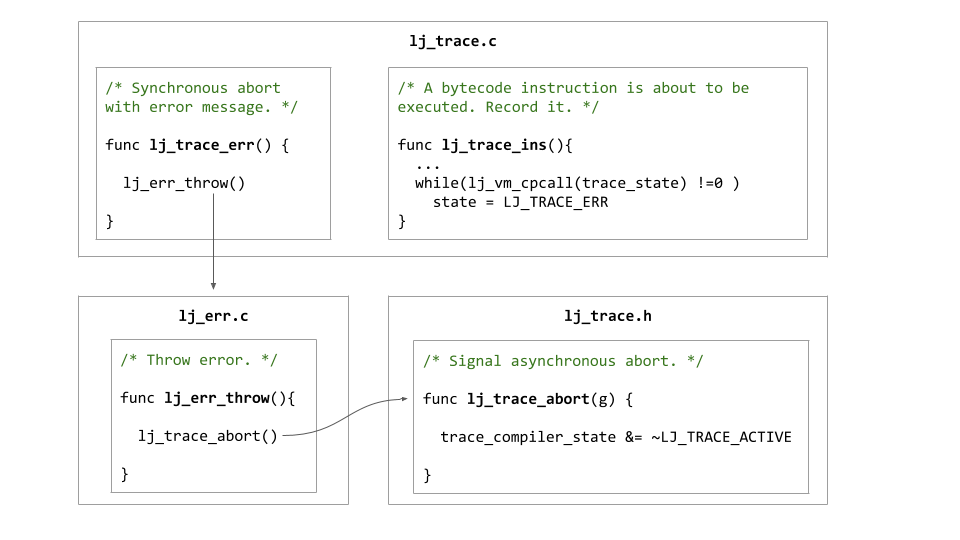
\includegraphics[width=\textwidth]{images/chapter7/throw_error.png}
    \caption{Throw error}
    \label{fig:throw-err}
\end{figure}

\begin{figure}[H]
    \centering
	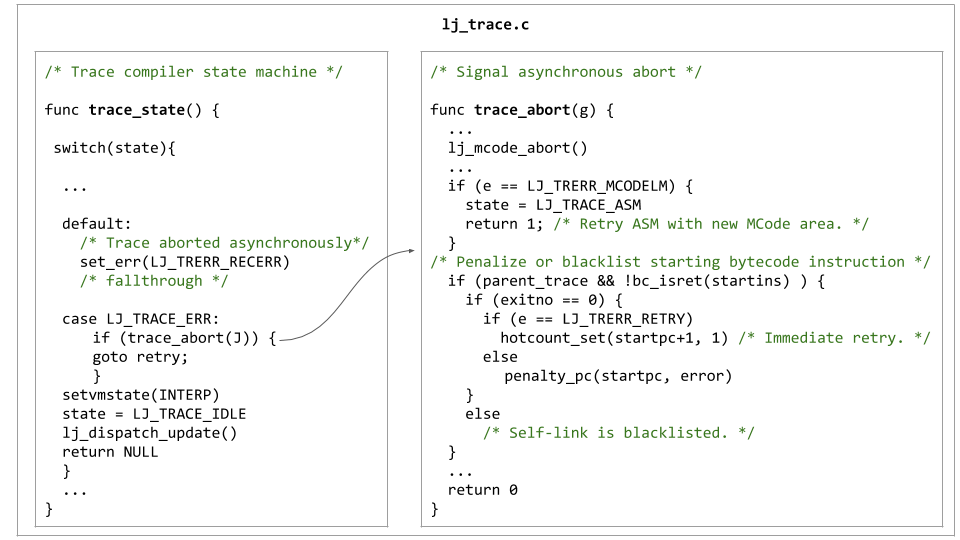
\includegraphics[width=\textwidth]{images/chapter7/abort.png}
    \caption{Abort}
    \label{fig:abort-mechanism}
\end{figure}


\noindent
Many aborts are influenced by the value of some parameters that users can set for the JIT compiler. The most important are shown in Tab. \ref{tab:parameters-jit}

\begin{center}
\begin{longtable}{|c|c|c|}
\hline
\textbf{Parameter} & \textbf{Deafult} & \textbf{Description}\\
\hline
maxtrace & 1000	 & Max. number of traces in the cache\\
maxrecord	 & 4000	 & Max. number of recorded IR instructions\\
maxirconst & 	500	   & Max. number of IR constants of a trace\\
maxside	 & 100	    & Max. number of side traces of a root trace\\
maxsnap & 	500	    & Max. number of snapshots for a trace\\
hotloop	 & 56	    & Number of iterations to detect a hotloop or hot call\\
hotexit	 & 10	    & Number of taken exits to start a side trace\\
tryside	 & 4	     & Number of attempts to compile a side trace\\
instunroll	 & 4	 & Max. unroll factor for instable loops\\
loopunroll & 	15   & Max. unroll factor for loop ops in side traces\\
callunroll	 & 3	 & Max. unroll factor for pseudo-recursive calls\\
recunroll	 & 2	 & Min. unroll factor for true recursion\\
sizemcode	 & 32	 & Size of each machine code area in KBytes (Windows: 64K)\\
maxmcode	 & 512	 & Max. total size of all machine code areas in KBytes\\
\hline
\caption{Parameters of the JIT compiler}
\label{tab:parameters-jit}
\end{longtable}
\end{center}


\subsection{Blacklisting}
\label{subsec:luajit-black}
LuaJIT implements blacklisting (see Sec. \ref{subsec:abort-blacklisting} for details) in order to prevent recording traces that it tried to generate, but it failed many times. 

When hotpath recording fails, the trace compiler increments a counter, so-called \textit{backoff} counter by Gal et al. \cite{gal2009trace}, linked to the hotcode that it tried to record unsuccessfully. Once this counter exceeds a certain threshold, the VM will never try to compile that hotcode again.

To avoid retrying compilation, the bytecode of the hotloop/hotfunction is patched with an operation that stops hotspot detection and force execution in the interpreter. Operations that force interpretation have the same syntax of 'standard' operation with \texttt{'I'} as prefix (see table \ref{tab:blacklistin-operations}).

\begin{table}[H]
    \centering
    \begin{tabular}{|c|c|c|}
        \hline
        'Standard' op & Force interpreter op & Description \\
        \hline
        \texttt{FORL} & \texttt{IFORL} & Numeric 'for' loop\\
        \texttt{LOOP} &  \texttt{ILOOP} & Generic loop\\
        \texttt{ITERL} & \texttt{IITERL} & Iterator 'for' loop\\
        \texttt{FUNCF} & \texttt{IFUNCF} & Fixed-arg Lua function\\
        \texttt{FUNCV} & \texttt{IFUNCV} & Vararg Lua function\\
        \hline
    \end{tabular}
    \caption{Bytecode instructions to force interpretation}
    \label{tab:blacklistin-operations}
\end{table}

\noindent
As mentioned, each time a trace aborts, the hotcode detected is penalised incrementing its \textit{backoff} counter. The penalty mechanism uses a 64-entries table defined into the JIT state. Each row contains: (i) the starting bytecode PC of the hotpath; (ii) the penalty value (previously called \textit{backoff} counter); (iii) the abort reason number (details in Tab. \ref{tab:abort-messages}). 

\begin{lstlisting}[style=CStyle, caption=\texttt{lj\_traceerr.h}]
/* Round-robin penalty cache for bytecodes leading to aborted traces. */
typedef struct HotPenalty {
  MRef pc;		/* Starting bytecode PC. */
  uint16_t val;		/* Penalty value, i.e. hotcount start. */
  uint16_t reason;	/* Abort reason (really TraceErr). */
} HotPenalty;

#define PENALTY_SLOTS	64	/* Penalty cache slot. Must be a power of 2. */
#define PENALTY_MIN	(36*2)	/* Minimum penalty value. */
#define PENALTY_MAX	60000	/* Maximum penalty value. */
#define PENALTY_RNDBITS	4	/* # of random bits to add to penalty value. */

/* JIT compiler state. */
typedef struct jit_State {
  ...
  HotPenalty penalty[PENALTY_SLOTS];  /* Penalty slots. */
  uint32_t penaltyslot;	/* Round-robin index into penalty slots. */
  uint32_t prngstate;	/* PRNG state. */
  ...
} jit_State;
\end{lstlisting}
\texttt{PENALTY\_MIN} represents the minimum increment of the counter and \texttt{PENALTY\_MAX} is the threshold for blacklisting. The variable \texttt{penaltyslot} is a round-robin index that points to the next available entry in the table. It is used when a new hotpath needs to be penalised. Tab. \ref{tab:hot-penalty-table} shows a snapshot of a hot penalty table as an example.
\begin{table}[H]
    \centering
    %\ttfamily
    \begin{tabular}{|c|c|c|c|}
        \hline
        Index & PC & val & reason \\
        \hline
        0 & \texttt{0x4157b014} & 55122 & 7\\
        1 & \texttt{0x41635430} & 56340 & 7\\ 
        2 & \texttt{0x41635070} & 1211 & 5\\ 
        3 & \texttt{0x4157b03c} & 
        617 & 10\\ 
        4 & \texttt{0} & 0 & 0 \\ 
        5 & \texttt{0} & 0 & 0\\ 
        ... & ... & ... & ...\\
        63 & \texttt{0} & 0 & 0\\
        \hline
    \end{tabular}
    \caption{Exemplifying snapshot of the Hot Penalty Table}
    \label{tab:hot-penalty-table}
\end{table}
\noindent
The penalisation mechanism is the following. When a trace aborts, the function \texttt{trace\_abort} is called. If the trace is a root trace, the PC of the starting bytecode instruction is penalized (thus the hotcode is penalised). The function \texttt{penalty\_pc} is responsible for the penalisation. If the penalty value exceeds the threshold (\texttt{PENALTY\_MAX}), the trace is blacklisted. Thus, the bytecode is patched with the adequate \texttt{I...} operation and the hotcode previously detected can never become hot again. In LuaJIT, blacklisting is permanent. Once a bytecode is blacklisted, it can never be whitelisted.

A description of penalisation and blacklisting is shown in the flow chart at Fig. \ref{fig:blacklisting}.
\begin{lstlisting}[style=CStyle, caption=\texttt{lj\_trace.c}]
/* Penalize a bytecode instruction. */
static void penalty_pc(jit_State *J, GCproto *pt, BCIns *pc, TraceError e) {
  uint32_t i, val = PENALTY_MIN;
  for (i = 0; i < PENALTY_SLOTS; i++)
    if (mref(J->penalty[i].pc, const BCIns) == pc) {  /* Cache slot found? */
      /* First try to bump its hotcount several times. */
      val = ((uint32_t)J->penalty[i].val << 1) + LJ_PRNG_BITS(J, PENALTY_RNDBITS);
      if (val > PENALTY_MAX) {
        @@blacklist_pc(pt, pc);@@  /* Blacklist it, if that didn't help. */
        return;
      }
      goto @@setpenalty@@;
    }
  /* Assign a new penalty cache slot. */
  i = J->penaltyslot;
  J->penaltyslot = (J->penaltyslot + 1) & (PENALTY_SLOTS-1);
  setmref(J->penalty[i].pc, pc);
  @@setpenalty:@@
  J->penalty[i].val = (uint16_t)val;
  J->penalty[i].reason = e;
  hotcount_set(J2GG(J), pc+1, val);
}

/* Blacklist a bytecode instruction. */
static void blacklist_pc(GCproto *pt, BCIns *pc) {
  setbc_op(pc, (int)bc_op(*pc)+(int)BC_ILOOP-(int)BC_LOOP);
  pt->flags |= PROTO_ILOOP;
}
\end{lstlisting}


\begin{figure}[H]
\hspace*{-1cm}
\begin{tikzpicture}[node distance=2.8cm, auto,]
  \tikzstyle{every state}=[rectangle, fill=none,draw=black,text=black]
  \node[state, rounded corners] (try_rec)   {try recording};
  \node[state, rounded corners]  (abort) [right= 2cm of try_rec] {abort};
  \node[state,align=center, rounded corners]  (succ_comp) [below of=try_rec] {successfully compiled\\patch BC with J...};
  \node[state, rounded corners]  (already_penalize) [right= 2cm of abort] {PC already penalized?};
  \node[state,align=center, rounded corners]  (new_entry) [below left of =already_penalize] {add new PC table entry:\\val = PENALTY\_MIN};
  \node[state,align=center, rounded corners]  (old_entry) [right= 1cm of new_entry] {increment PC penalty val:\\val = val + small\_rand\_num\\is val > PENALTY\_MAX?};
  \node[state,align=center, rounded corners]  (no_black) [below of =new_entry] {retry recording if\\the same hotspot\\ is detected again};
  \node[state,align=center, rounded corners]  (yes_black) [below of =old_entry] {blacklist hotcode\\patch BC with I...};
  
  \draw[->] (try_rec) -- (abort) node[near start, shift={(0.5,0)}] {fail};
  \draw[->] (try_rec) -- (succ_comp) node[near start, shift={(-0.7,-0.5)}] {ok};
  \draw[->] (abort) -- (already_penalize);
  \draw[->] (already_penalize) -- (new_entry) node[near start, shift={(-0.9,+0.1)}] {no};
  \draw[->] (already_penalize) -- (old_entry) node[near start, shift={(+0.4,-0.4)}] {yes};
  \draw[->] (new_entry) -- (no_black);
  \draw[->] (old_entry) -- (no_black) node[near start, shift={(-0.3,-0.2)}] {no};
  \draw[->] (old_entry) -- (yes_black) node[near start, shift={(0.1,-0.4)}] {yes};
  \draw[->] (no_black) -- (try_rec);
  
\end{tikzpicture}
\caption{Penalization and blacklisting}
\label{fig:blacklisting}
\end{figure}

\begin{comment}
  \node[state] (IDLE)   {IDLE};
  \node[state]  (START) [right=2 cm of IDLE] {START};
  \node[state]  (RECORD) [right=2 cm of START] {RECORD};
  \node[state]  (END) [right of=RECORD] {END};
  \node[state]  (ASM) [right of=END] {ASM};
  \node[state]  (ERR) [below of=RECORD] {ERR};
    
  \path (IDLE)      edge node {new trace} (START)
        (START)     edge node {start rec} (RECORD)
        (RECORD)    edge node {stop rec} (END)
        (RECORD)   edge node {abort} (ERR)
        (END)       edge node {assemble} (ASM)
        (RECORD)    [loop above] edge node [shift={(1.3,-0.6)}] {rec next ins} (RECORD)
        (ASM)   [bend right] edge node  {trace successfully compiled} (IDLE)
        (ERR)   [bend left] edge node [shift={(-0.7,-0.7)}] {error detected} (IDLE)
        (END)   [bend left] edge node  [shift={(0.5,-0.5)}] {abort} (ERR)
        (ASM)   [bend left] edge node  [shift={(0.5,-0.5)}] {abort} (ERR);
\end{comment}

\noindent
Differently from the hotcount mechanism, collisions can never occur in the hot penalty table. The PC is used to check if a hotcode has already been penalized. Since the PC (that contains the memory address of the current bytecode instruction) is unique, collisions are impossible.

However, another small drawback can occur because of the round-robin index. When there are enough traces aborts after each other so that the hot penalty table is full (the 64 slots are already taken by ongoing penalised bytecode), a slot can be reused before its counter gets high enough to cause blacklisting. Thus, the next abort of the trace linked to the overwritten counter will be considered as its previous count was discarded. The trace compiler will link that hotpath to a different slot, as if it never aborted before. 

The probability of ending up in such an inconvenient situation is relatively low. In fact, Mike Pall commented this issue on the LuaJIT mailing list saying: \textit{"While theoretically possible, I've never seen this happen. In practice, something does get blacklisted eventually, which frees up a penalty tracking slot. There are only ever a handful of these slots in use. 64 slots is really generous"}\footnote{Conversation on the LuaJIT mailing list: \texttt{https://www.freelists.org/post/luajit/\\When-to-turn-off-JIT,4}}.

% When the recording of the hotcode related to the overwritten slot aborts again, 

\subsubsection{Blacklisting cancer}
Blacklisting is a very powerful tool that is used in the context of LuaJIT to save time avoiding to retry compilation of hotpaths that aborted repeatedly.  However, a really unpleasant situation can arise as a consequence of the fact that in LuaJIT blacklisting is permanent. In other words, blacklisted fragments of code cannot be whitelisted ever again. On one hand, this is reasonable because there is no sense in recording a trace that contains a code fragment which failed to compile many times (hence it was blacklisted). On the other hand, it could be possible that the same code fragment can be successfully compiled in a different context of a new trace.

Moreover, LuaJIT blacklists hotpaths that hits an already blacklisted code fragment. To be more precise, if the interpreter hits an already blacklisted bytecode instruction (\texttt{I...}) while recording a new trace, trace creation is aborted and the new trace is also blacklisted. This could lead to a mechanism of \textit{cascading blacklisting} from a code fragment to another. It is particularly dangerous when LuaJIT blacklists a key function of an application (i.e. a function called in many points of the source code) because the cascade of blacklisting spreads rapidly all over the code, hence the name \textit{blacklisting cancer}. 

To not fall is such an inconvenient situation we should avoid to use programming patterns which emphasise this problem. An exemplifying situation on this subject was discussed in the LuaJIT community\footnote{Conversation on the LuaJIT mailing list: 
\texttt{https://www.freelists.org/post/luajit/\\ANN-dumpanalyze-tool-for-working-with-LuaJIT-dumps,12}}. This example is proposed again below to better illustrate the problem.

\newpage

\begin{lstlisting}[style=LuaStyle]
-- Blacklisting Cancer 

-- Call a function with an argument.
local function apply (f, x) 
	return f(x)
end

-- Return the value x wrapped inside a closure.
local function fwrap (x)
   return function () return x end -- Create a closure Not-Yet-Implemented (NYI)
end

-- Attempt to compile that naturally fails. 
for i=1,1e5 do 
	apply(fwrap, i) -- Abort message: NYI: create a closure
end

-- apply() function is now permanently blacklisted.
-- Every call to apply() in the future will have to be run by the interpreter.

local function nop (x) 
end

-- Attempt to compile that should not fail.
for i=1,1e5 do
	apply(nop, i) -- Abort message: calling blacklisted function
end
\end{lstlisting}

\noindent
The JIT permanently blacklists \texttt{apply()}. It will never allow that function to be called in a trace. In fact, the second loop could have been compiled successfully if it was run before the first loop.

It should be mention that other implementations of tracing JIT do not suffer from this problem. For instance, RaptorJIT \cite{gorrie2017raptorjit} gives another chance to blacklisted code fragments of being compiled in a different context. In particular, when calling a blacklisted function from JIT code, it ignores the blacklisting and it just inline the content of the function. It tries to compile the function in the context of its caller. It can be worth to do it because sometimes code fails to compile in isolation, but a function can be compiled in the context of its caller. In fact, this implies overhead, since RaptorJIT puts more effort to generate machine code at the expense of making more compilation attempts.

% **** Snapshots ****
\section{Snapshots}
\label{sec:snapshots}
Snapshot is a key feature used in LuaJIT to leave the VM in a consistent state when a trace exits. When the execution leaves a trace because of guard failures, the system switches to interpretation. The VM should be left in a consistent state for the interpret to continue. This means that all updates (stores) to the state (stack or objects) must track the original language semantics. In particular the values held in registers throughout the trace must be written to their respective stack locations. Once the stack is in a suitable state, the interpreter can continue.

Within the possible techniques used in trace-based just-in-time compilation (see Sec. \ref{subsec:trace-exit}), LuaJIT solves the problem of keeping the VM in a consistent state by maintaining a mapping from stack location to SSA IR instructions. Such mappings are called \textit{snapshots} in the LuaJIT codebase. Using a snapshot, LuaJIT can then reconstruct the operand stack as it would have been if the instructions in the trace were interpreted.

The Snapshot mechanism is implemented in the \texttt{lj\_snap.[c,h]}, and the \texttt{SnapShot} data structure is defined in \texttt{lj\_jit.h} (the key functions are \texttt{lj\_snap\_restore} and \texttt{snap\_restoreval}).

Snapshots can be see at the IR level. From the definition in the official LuaJIT website \cite{luajit-ir}: a snapshot captures the IR references corresponding to modified slots and frames in the bytecode execution stack. Every snapshot saves a specific bytecode execution state, which can later be restored on trace exits. Snapshots are sparsely emitted and compressed. Snapshots provide the link between the IR and the bytecode domain (and transitively the source code domain, via the bytecode debug info).

Code sinking via snapshots allows sinking of arbitrary code without the overhead of the other approaches. A snapshot stores a consistent view of all updates to the state before an exit. If an exit is taken the on-trace machine state (registers and spill slots) and the snapshot can be used to restore the VM state.

The snapshot mechanism is slow if compared to other approaches such as \textit{exit stubs} (see Sec. \ref{subsec:trace-exit}), but this should be seen as a problem in LuaJIT. By quoting Mike Pall in \cite{luajit-mail-1} \textit{"State restoration using this data-driven approach is slow of course. But repeatedly taken side exits quickly trigger the generation of side traces. The snapshot is used to initialise the IR of the side trace with the necessary state using pseudo-loads. These can be optimised together with the remainder of the side trace. The pseudo-loads are unified with the machine state of the parent trace by the back-end to enable zero-cost linking to side traces"}.
  
\subsection{Example}
Here we propose a concrete example which describes snapshots.
\begin{mdframed}[style=LuaStyleFrame]
\begin{lstlisting}[style=LuaStyle]
-- Snapshot

local x = 0

-- A for loop implicitly define tacit variables: 
-- index i (intern), limit N, step s, index i (extern)
for i=1,200 do
	if i < 100 then x = x + 11
	else x = x + 22 end
end
\end{lstlisting}
\end{mdframed}
\noindent
LuaJIT stores the local variables in stack slots according to the order in which they appear in the code. When a local variable is declared, a single slot is reserved to store it. On the other hand, a \texttt{for} loop reserves 4 slots that contain respectively: (i) the internal copy of the index, (ii) the limit of the loop, (iii) the step of each iteration and (iv) the external copy of the index. See Tab. \ref{tab:snap-var-alloc} for details.
\begin{table}[H]
    \centering
    \begin{tabular}{|c|c|c|c|}
        \hline
        Stack slot number & Variable & Type & Structure\\
        \hline
        \texttt{\#0} & - & - & closure/frame slot\\
        \hline
        \texttt{\#1} &  \texttt{x} & local var & declaration\\
        \hline
        \texttt{\#2} & \texttt{i} & index \footnotesize{(internal copy)} & \multirow{4}{*}{loop} \\
        \texttt{\#3} & \texttt{N} & limit & \\
        \texttt{\#4} & \texttt{s} & step & \\
        \texttt{\#5} & \texttt{i} & index \footnotesize{(external copy)} & \\
        \hline
    \end{tabular}
    \caption{Slots variables allocation}
    \label{tab:snap-var-alloc}
\end{table}
\noindent
When printing the IR through \texttt{jdump} you can visualise snapshots by selecting the flag '\texttt{s}'. A typical use of this option is shown below. 
\begin{lstlisting}[style=DumpStyle]
   ./luajit -jdump=is Ex.lua
\end{lstlisting}
\noindent
Once you manage to print snapshots in the IR you should be aware that:
\begin{center}
    \textbf{Each snaphot (SNAP) lists the modified stack slots and their values. The \textit{i-th} value in the snapshot list represents the index of the IR that writes a value in slot number \texttt{\#i}; "\texttt{----}" indicates that the slot is not written. Frames are separated by "\texttt{|}".}
\end{center}
Going back to the example previously desbribe the corresponding IR is the following.
\begin{lstlisting}[style=DumpStyle]
---- TRACE 1 start Ex.lua:7
---- TRACE 1 IR
....        SNAP   #0   [ ---- ]
0001    int SLOAD  #2    CI
0002 >  num SLOAD  #1    T
0003  + num ADD    0002  +11 
0004  + int ADD    0001  +1  
....        SNAP   #1   [ ---- 0003 ]
0005 >  int LE     0004  +100
....        SNAP   #2   [ ---- 0003 0004 ---- ---- 0004 ]
0006 ------ LOOP ------------
0007  + num ADD    0003  +11 
0008  + int ADD    0004  +1  
....        SNAP   #3   [ ---- 0007 ]
0009 >  int LE     0008  +100
0010    int PHI    0004  0008
0011    num PHI    0003  0007
---- TRACE 1 stop -> loop
\end{lstlisting}
In this example slot \texttt{\#0} is not written since the frame slot doesn't change. In \texttt{SNAP \#1} the value of x changes because we compute \texttt{x=x+11}, hence the IR at index \texttt{0003} writes a value in slot \texttt{\#1}. \texttt{SNAP \#2} stores the changes of x as before and it stores the value of \texttt{i} because it was incremented \texttt{i=i+1} and it is checked that \texttt{i$<$100}. In this case the IR at index \texttt{0004} writes a value in slot \texttt{\#2} and \texttt{\#5} (internal and external copy of the index). \texttt{SNAP \#3} is the same of \texttt{SNAP \#1} but it considers the IR at index \texttt{0007}.

\subsection{Sparse snapshots}
As previously mentioned when a guard fails the trace is exited and the VM must be in a consistent state. This is achieved through snapshots, but LuaJIT avoids generating a snapshot for each guard of a trace. Guards that have a low probability of being wrongly predicted do not cause snapshots. This is a feature of LuaJIT called \textit{sparse snapshot} by Mike Pall. Here we propose his explanation about it presented in the LuaJIT 2.0 intellectual property disclosure and research opportunities \cite{luajit-mail-1}.

\textit{"Taking a full snapshot of all state updates before every exit would need a considerable amount of storage. Since all scalar stores are sunk, it's feasible to reduce the snapshot density. The basic idea is that it doesn't matter which state is restored on a taken exit, as long as it's consistent.}

\textit{This is a form of transactional state management. Every snapshot is a commit; a taken exit causes a rollback to the last commit. The on-trace state may advance beyond the last commit as long as this doesn't affect the possibility of a rollback. In practice this means that all on-trace updates to the state (non-scalar stores that are not sunk) need to force a new snapshot for the next exit.}

\textit{Otherwise the trace recorder only generates a snapshot after control-flow constructs that are present in the source, too. Guards that have a low probability of being wrongly predicted do not cause snapshots (e.g. function dispatch). This further reduces the snapshot density. Sparse snapshots also improve on-trace code quality, because they reduce the live range of the results of intermediate computations. Scheduling decisions can be made over a longer stream of instructions, too"}.

% **** Variables allocation ****
\section{Variables allocation}

\begin{comment}
\begin{multicols}{2}
\noindent
\textbf{Prerequisites}\\
To read this chapter you are supposed to know: what is a tracing JIT; the mechanism of traces and side traces; what are SSA intermediate representation (IR) and bytecode (see Chapter \ref{}).

\columnbreak
\noindent
\textbf{What you want to learn}\\
After reading this chapter you will learn how LuaJIT handles variables allocation.
\end{multicols}
\end{comment}
The aim of this section is to describe how variables are allocated in the bytecode and in the SSA IR. In particular, (i) the first paragraph investigates the allocation of local variables, (ii) the second paragraph considers the case of global variables and (iii) the last paragraphs examines upvalues. In each of them it will be shown an example that clarifies what explained.

\subsection{Local variables}

\begin{comment} %% -------------------------------

\subsection{Loop}
\begin{mdframed}[style=LuaStyleFrame]
\begin{lstlisting}[style=LuaStyle]
-- Loop with local variables

local x = 0
local N = 1e3
local s = 1

for i=1,N,s do
	x = x + 11
end
\end{lstlisting}
\end{mdframed}

\noindent
Bytecode
\begin{lstlisting}[style=DumpStyle]
---- TRACE 1 start Ex.lua:7
0008  ADDVN    0   0   0  ; 11
0009  FORL     3 => 0008
---- TRACE 1 stop -> loop

\end{lstlisting}

\noindent
IR

\begin{multicols}{2}
\begin{lstlisting}[style=DumpStyle]
---- TRACE 1 start Ex.lua:7
---- TRACE 1 IR
0001 rax   >  int SLOAD  #5    CRI
0002 rcx   >  int SLOAD  #6    CRI
0003       >  int GE     0002  +0  
0004 rbx   >  int ADDOV  0002  0001
0005          int USE    0004
0006 rbp      int SLOAD  #4    CI
0007 xmm7  >  num SLOAD  #1    T
0008 xmm7   + num ADD    0007  +11 
0009 rbp    + int ADD    0006  0002
0010       >  int LE     0009  0001
0011 ------------ LOOP ------------
0012 xmm7   + num ADD    0008  +11 
0013 rbp    + int ADD    0009  0002
0014       >  int LE     0013  0001
0015 rbp      int PHI    0009  0013
0016 xmm7     num PHI    0008  0012
---- TRACE 1 stop -> loop
\end{lstlisting}
\end{multicols}

\begin{table}[H]
    \centering
    \begin{tabular}{|c|c|c|c|}
        \hline
            Structure & Type & Variable & Stack slot number\\
        \hline
        \multirow{3}{*}{initialisation} & local var & \texttt{x} & \texttt{\#1} \\
        & local var & \texttt{N} & \texttt{\#2} \\
        & local var & \texttt{s} & \texttt{\#3} \\
        \hline
        \multirow{4}{*}{loop} & index \footnotesize{(internal copy)} & \texttt{i} & \texttt{\#4} \\
        & limit & \texttt{N} & \texttt{\#5} \\
        & step & \texttt{s} & \texttt{\#6} \\
        & index \footnotesize{(external copy)} & \texttt{i} & \texttt{\#7} \\
        \hline
    \end{tabular}
    \caption{Table}
    \label{tab:my_label}
\end{table}

\subsection{Nested loop}

\end{comment}

Local variables are stored in stack slots according to the order they appear in the code. When a local variable is declared, a single slot is reserved to store it. On the other hand, a \texttt{for} loop reserves 4 slots that contain respectively: (i) the internal copy of the index, (ii) the limit of the loop, (iii) the step of each iteration and (iv) the external copy of the index. 
\begin{mdframed}[style=LuaStyleFrame]
\begin{lstlisting}[style=LuaStyle]
-- Nested loop with local variables

local iN, iS = 1e3, 2   -- i limit, step
local jN, jS = 1e4, 3   -- j limit, step

for i=1,iN,iS do        -- outer loop
  local x = 0
  for j=1,jN,jS do      -- inner loop
    i = i + 1
    x = x + i
  end
end
\end{lstlisting}
\end{mdframed}

\noindent
The example above contains in order: variables declaration (line \texttt{4}), for loop (line \texttt{6}), variable declaration (line \texttt{7}), for loop (line \texttt{8}). Thus, variables will be allocated in order in the stack slots as show in table \ref{tab:allocation-local}.

\begin{table}[H]
    \centering
    \begin{tabular}{|c|c|c|c|}
        \hline
            Structure & Type & Variable & Stack slot number\\
        \hline
        \multirow{4}{*}{declaration} & local var & \texttt{iN} & \texttt{\#1} \\
        & local var & \texttt{iS} & \texttt{\#2} \\
        & local var & \texttt{jN} & \texttt{\#3} \\
        & local var & \texttt{jS} & \texttt{\#4} \\
       
        \hline
        \multirow{4}{*}{outer loop} & index \footnotesize{(internal copy)} & \texttt{i} & \texttt{\#5}\\
        & limit & \texttt{iN} & \texttt{\#6} \\
        & step & \texttt{iS} & \texttt{\#7} \\
        & index \footnotesize{(external copy)} & \texttt{i} & \texttt{\#8} \\
        \hline
        declaration & local var & \texttt{x} & \texttt{\#9} \\
        \hline
        \multirow{4}{*}{inner loop} & index \footnotesize{(internal copy)} & \texttt{j} & \texttt{\#10}\\
        & limit & \texttt{jN} & \texttt{\#11} \\
        & step & \texttt{jS} & \texttt{\#12} \\
        & index \footnotesize{(external copy)} & \texttt{j} & \texttt{\#13} \\
        \hline
    \end{tabular}
    \caption{Local variables allocation}
    \label{tab:allocation-local}
\end{table}

\begin{comment}
\noindent
Bytecode

\begin{multicols}{2}
\begin{lstlisting}[style=DumpStyle]
---- TRACE 1 start Ex.lua:8
0014  ADDVN    7   7   0  ; 1
0015  ADDVV    8   8   7
0016  FORL     9 => 0014
---- TRACE 1 stop -> loop

---- TRACE 2 start 1/3 Ex.lua:6
0017  FORL     4 => 0009
0009  KSHORT   8   0
0010  KSHORT   9   1
0011  MOV     10   2
0012  MOV     11   3
0013  JFORI    9 => 0017
---- TRACE 2 stop -> 1
\end{lstlisting}
\end{multicols}

\end{comment}

\noindent
Below it is shown the IR dump. Variables are loaded with the \texttt{SLOAD} (stack slot load) operation where the left operand  \texttt{\#}\textit{n} refers to the variable slot number and the right operand contains flags (see \ref{} for details about flags).

\begin{multicols}{2}
\begin{lstlisting}[style=DumpStyle]
---- TRACE 1 start Ex.lua:8
---- TRACE 1 IR
0001 rax   >  int SLOAD  #11   CRI
0002 rcx   >  int SLOAD  #12   CRI
0003       >  int GE     0002  +0  
0004 rbx   >  int ADDOV  0002  0001
0005          int USE    0004
0006 rbp      int SLOAD  #10   CI
0007 xmm6  >  num SLOAD  #8    T
0008 xmm6   + num ADD    0007  +1  
0009 xmm7  >  num SLOAD  #9    T
0010 xmm7   + num ADD    0009  0008
0011 rbp    + int ADD    0006  0002
0012       >  int LE     0011  0001
0013 ------------ LOOP ------------
0014 xmm6   + num ADD    0008  +1  
0015 xmm7   + num ADD    0014  0010
0016 rbp    + int ADD    0011  0002
0017       >  int LE     0016  0001
0018 rbp      int PHI    0011  0016
0019 xmm6     num PHI    0008  0014
0020 xmm7     num PHI    0010  0015
---- TRACE 1 stop -> loop

---- TRACE 2 start 1/3 Ex.lua:6
---- TRACE 2 IR
0001 xmm6     num SLOAD  #8    PI
0002 xmm7     num SLOAD  #9    PI
0003 xmm2     num SLOAD  #6    RI
0004 xmm1     num SLOAD  #7    RI
0005       >  num GE     0004  +0  
0006 xmm7     num SLOAD  #5    I
0007 xmm7     num ADD    0006  0004
0008       >  num LE     0007  0003
0009 xmm4  >  num SLOAD  #3    T
0010 xmm3  >  num SLOAD  #4    T
0011 rbp   >  int CONV   0009  int.num
0012 rbx   >  int CONV   0010  int.num
0013       >  int GE     0012  +0  
0014 rbx   >  int ADDOV  0012  0011
0015          int USE    0014
0016       >  int GE     0011  +1  
---- TRACE 2 stop -> 1

\end{lstlisting}
\end{multicols}

\noindent
Note that \texttt{\#0} indicates the closure/frame slot and \texttt{\#1} the first variable slot (corresponding to slot \texttt{0} of the bytecode). Moreover, there are no store operations for stack slots. When the execution flow exits from a trace, values on stack slots are restored. All stores to stack slots are effectively sunk into exits or side traces \cite{luajit-ir}.

\subsection{Global variables}
Dealing with global variables is more subtle because their value can be modified from different part of the code. In fact, the concept of global variables does not exist explicitly in Lua. To preserve the illusion of global variables, Lua keeps them internally in a regular table that is used as \textit{global environment} (this is a simplification of what really occurs, see \cite{lua-book-chapter22} for more details). 

\begin{comment} %% --------------------------------------------------

\begin{mdframed}[style=LuaStyleFrame]
\begin{lstlisting}[style=LuaStyle]
-- Loop with global variable

x = 0

for i=1,1e3 do
	x = x + 11
end
\end{lstlisting}
\end{mdframed}

\noindent
Bytecode
\begin{lstlisting}[style=DumpStyle]
---- TRACE 1 start variables_global.lua:5
0007  GGET     4   0      ; "x"
0008  ADDVN    4   4   0  ; 11
0009  GSET     4   0      ; "x"
0010  FORL     0 => 0007
---- TRACE 1 stop -> loop
\end{lstlisting}

\noindent
IR

\begin{multicols}{2}
\begin{lstlisting}[style=DumpStyle]
---- TRACE 1 start Ex.lua:5
---- TRACE 1 IR
0001 rbp      int SLOAD  #1    CI
0002 rbx      fun SLOAD  #0    R
0003 rdx      tab FLOAD  0002  func.env
0004          int FLOAD  0003  tab.hmask
0005       >  int EQ     0004  +63 
0006 rcx      p32 FLOAD  0003  tab.node
0007 rax   >  p32 HREFK  0006  "x"  @33
0008 xmm7  >  num HLOAD  0007
0009 xmm7   + num ADD    0008  +11 
0010          num HSTORE 0007  0009
0011 rbp    + int ADD    0001  +1  
0012       >  int LE     0011  +1000
0013 ------------ LOOP ------------
0014 xmm7   + num ADD    0009  +11 
0015          num HSTORE 0007  0014
0016 rbp    + int ADD    0011  +1  
0017       >  int LE     0016  +1000
0018 rbp      int PHI    0011  0016
0019 xmm7     num PHI    0009  0014
---- TRACE 1 stop -> loop
\end{lstlisting}
\end{multicols}


%%%%%%%%%%%%%%%%%%%%%%%%%%%%%%%

\begin{mdframed}[style=LuaStyleFrame]
\begin{lstlisting}[style=LuaStyle]
-- Loop with global variable

y = 0 

for i=1,1e3 do
	y = 11
end
\end{lstlisting}
\end{mdframed}

\noindent
Bytecode

\begin{lstlisting}[style=DumpStyle]
---- TRACE 1 start variables_global.lua:5
0007  KSHORT   4  11
0008  GSET     4   0      ; "y"
0009  FORL     0 => 0007
---- TRACE 1 stop -> loop
\end{lstlisting}


\noindent
IR

\begin{multicols}{2}
\begin{lstlisting}[style=DumpStyle]
---- TRACE 1 start Ex.lua:5
---- TRACE 1 IR
0001 rbp      int SLOAD  #1    CI
0002 rdx      fun SLOAD  #0    R
0003 rax      tab FLOAD  0002  func.env
0004          int FLOAD  0003  tab.hmask
0005       >  int EQ     0004  +63 
0006 rcx      p32 FLOAD  0003  tab.node
0007       >  p32 HREFK  0006  "y"  @34
0008          tab FLOAD  0003  tab.meta
0009       >  tab EQ     0008  NULL
0010          num HSTORE 0007  +11 
0011          nil TBAR   0003
0012 rbp    + int ADD    0001  +1  
0013       >  int LE     0012  +1000
0014 ------------ LOOP ------------
0015 rbp    + int ADD    0012  +1  
0016       >  int LE     0015  +1000
0017 rbp      int PHI    0012  0015
---- TRACE 1 stop -> loop
\end{lstlisting}
\end{multicols}

\end{comment}


\begin{mdframed}[style=LuaStyleFrame]
\begin{lstlisting}[style=LuaStyle]
-- Loop with global variables

x, y = 0, 0

for i=1,1e3 do
	x = x + 11
	y = 22
end
\end{lstlisting}
\end{mdframed}

\noindent
The example contains two global variables \texttt{x} and \texttt{y}. The value of \texttt{x} is updated at each iteration of the loop, while \texttt{y} can be moved outside the body of the loop by LICM without affecting the semantic of the program. As expected this optimisation is performed only at IR level, but not in the bytecode.

\begin{multicols}{2}
\begin{lstlisting}[style=DumpStyle]
---- TRACE 1 start Ex.lua:5
0009  GGET     4   1      ; "x"
0010  ADDVN    4   4   0  ; 11
0011  GSET     4   1      ; "x"
0012  KSHORT   4  22
0013  GSET     4   0      ; "y"
0014  FORL     0 => 0009
---- TRACE 1 stop -> loop
\end{lstlisting}
\end{multicols}

\noindent
As shown in the bytecode above, \texttt{x} and \texttt{y} are retrieved and modified with the instructions \texttt{GGET} (global get) and \texttt{GSET} (global set) because they are global variables.

In the IR it is possible to see more details of what really occurs.

\begin{multicols}{2}
\begin{lstlisting}[style=DumpStyle]
---- TRACE 1 start Ex.lua:5
---- TRACE 1 IR
0001 rbp      int SLOAD  #1    CI
0002 rbx      fun SLOAD  #0    R
0003 rcx      tab FLOAD  0002  func.env
0004          int FLOAD  0003  tab.hmask
0005       >  int EQ     0004  +63 
0006 rdx      p32 FLOAD  0003  tab.node
0007 rax   >  p32 HREFK  0006  "x"  @33
0008 xmm7  >  num HLOAD  0007
0009 xmm7   + num ADD    0008  +11 
0010          num HSTORE 0007  0009
0011       >  p32 HREFK  0006  "y"  @34
0012          tab FLOAD  0003  tab.meta
0013       >  tab EQ     0012  NULL
0014          num HSTORE 0011  +22 
0015          nil TBAR   0003
0016 rbp    + int ADD    0001  +1  
0017       >  int LE     0016  +1000
0018 ------------ LOOP ------------
0019 xmm7   + num ADD    0009  +11 
0020          num HSTORE 0007  0019
0021 rbp    + int ADD    0016  +1  
0022       >  int LE     0021  +1000
0023 rbp      int PHI    0016  0021
0024 xmm7     num PHI    0009  0019
---- TRACE 1 stop -> loop
\end{lstlisting}
\end{multicols}

\noindent
\texttt{SLOAD} at line \texttt{0001} refers to the variable \texttt{i} and \texttt{SLOAD} at line \texttt{0002} is relative to the starting frame of the trace, where \texttt{\#0} indicates the frame slot. Then, \texttt{FLOAD} (object field load) at line \texttt{0003} accesses the global environment (\texttt{func.env}). At line \texttt{0004} the size of the hash part (\texttt{tab.hmask}) is loaded and at line \texttt{0005} it is checked that its value is not changed (\texttt{hmask=+63}). Finally, the table hash part (\texttt{tab.node}) is loaded  at line \texttt{0006} and with \texttt{HREFK} (constant hash reference) \texttt{"x"} is retrieved from the global environment table (line \texttt{0007}). Once the reference has been retrieved the value of \texttt{x} is loaded with \texttt{HLOAD} (line \texttt{0008}) and stored with \texttt{HSTORE} (line \texttt{0010} and \texttt{0020}).

Since the global environment has already been loaded, there is no need to do it again for \texttt{y}. Thus, \texttt{"y"} can be retrieved with \texttt{HREFK} (line \texttt{0011}). Then, the global environment metatable is loaded (line \texttt{0012}) and it is checked that it is equal to \texttt{NULL} (line \texttt{0013}). After storing the value of \texttt{y} with \texttt{HSTORE} (line \texttt{0014}) the compiler creates a table write barrier (line \texttt{0015}). \texttt{TBAR} (table write barrier) is a write barrier needed for the incremental garbage collector.

%%%%%%%%%%%%%%%%%%%%%%%%%%%%%%%%%%%%%%%%%%%%%%%%%%%55
\subsection{Upvalues}
Closure and upvalues are a key concept in Lua. Thus, LuaJIT has specific instructions to handle them both at bytecode and IR level.

The example below shows a loop with a closure that contains an upvalue: the closure is inlined in the trace and the upvalue is modified inside it.
\begin{mdframed}[style=LuaStyleFrame]
\begin{lstlisting}[style=LuaStyle]
-- Recursive function with upvalue

local function f(x)
  return function(y)    -- return a closure
    x = x + 1
    return x + y
  end
end

local a = 0
local b = f(0)

for i=1,1e3 do
	a = b(i) + 2
end
\end{lstlisting}
\end{mdframed}

\noindent
In the bytecode below it is possible to see the fact that the closure is inlined (lines \texttt{0000-00006}). The dot in the second column of the bytecode represents the depth in the call. What is interesting is the fact that the upvalue \texttt{x} is retrieved and modified with the instructions \texttt{UGET} (get upvalue) and \texttt{USETV} (set upvalue to variable).

\begin{multicols}{2}
\begin{lstlisting}[style=DumpStyle]
---- TRACE 1 start Ex.lua:13
0010  MOV      7   2
0011  MOV      8   6
0012  CALL     7   2   2
0000  . FUNCF    2          ; Ex.lua:4
0001  . UGET     1   0      ; x
0002  . ADDVN    1   1   0  ; 1
0003  . USETV    0   1      ; x
0004  . UGET     1   0      ; x
0005  . ADDVV    1   1   0
0006  . RET1     1   2
0013  ADDVN    1   7   0  ; 2
0014  FORL     3 => 0010
---- TRACE 1 stop -> loop
\end{lstlisting}
\end{multicols}

\noindent
The same mechanism is shown in the IR.

\begin{multicols}{2}
\begin{lstlisting}[style=DumpStyle]
---- TRACE 1 start Ex.lua:13
---- TRACE 1 IR
0001 rbp      int SLOAD  #4    CI
0002       >  fun SLOAD  #3    T
0003       >  fun EQ     0002  Ex.lua:4
0004       >  p32 UREFC  Ex.lua:4  #0  
0005 xmm6  >  num ULOAD  0004
0006 xmm6   + num ADD    0005  +1  
0007          num USTORE 0004  0006
0008 xmm7     num CONV   0001  num.int
0009 xmm7     num ADD    0008  0006
0010 xmm7   + num ADD    0009  +2  
0011 rbp    + int ADD    0001  +1  
0012       >  int LE     0011  +1000
0013 ------------ LOOP ------------
0014 xmm6   + num ADD    0006  +1  
0015          num USTORE 0004  0014
0016 xmm7     num CONV   0011  num.int
0017 xmm7     num ADD    0016  0014
0018 xmm7   + num ADD    0017  +2  
0019 rbp    + int ADD    0011  +1  
0020       >  int LE     0019  +1000
0021 rbp      int PHI    0011  0019
0022 xmm6     num PHI    0006  0014
0023 xmm7     num PHI    0010  0018
---- TRACE 1 stop -> loop
\end{lstlisting}
\end{multicols}

\noindent
\texttt{SLOAD} at line \texttt{0001} refers to the variable \texttt{i} and \texttt{SLOAD} at line \texttt{0002} loads the closure assigned to the variable \texttt{b}. Then it is checked that the closure loaded is equal to what is returned at \texttt{Ex.lua:4} (line \texttt{0003}). \texttt{UREFC} (closed upvalue reference) gets the upvalue reference from the closure (line \texttt{0004}). Finally, it is possible to load and store the upvalue with \texttt{ULOAD} (line \texttt{0005}) and \texttt{USTORE} (line \texttt{0007} and \texttt{0015}).
 

\iffalse

\subsection{Loop with assignment and global variable}
This example has been designed to analyse what happens if the loop contains variable assignments in the case of global or local variables. Moreover, it will be shown that the compiler is able to move invariant instructions out of loops \cite{lj-mail-understand-ir}. It performs the traditional loop-invariant code motion (LICM) optimisation. Another small difference from the previous example is that the maximum loop counter is not a literal but it is a variable ($N=100$). 
\begin{mdframed}[style=LuaStyleFrame]
\begin{lstlisting}[style=LuaStyle]
-- Loop with assignment

y = 0
local x = 0
local N = 100

for i=1,N do
	 y = 2      -- global variable assignment
	 x = x+3    -- local variable assignment
end
\end{lstlisting}
\end{mdframed}

\noindent
As shown in the bytecode below, the fact that \texttt{y} is a global variable implies the \texttt{GSET} instruction ('global' set) when doing the assignment $y=2$. Then, \texttt{ADDVN} simply computes the $x=x+3$ operation. 

Here it is clear that at bytecode level the LICM optimisation is not applied because the execution flow makes a backward jump to line \texttt{0009} and $y=2$ is repeated at each iteration of the loop. In fact, no optimisation is performed by LuaJIT on bytecode.

\begin{lstlisting}[style=DumpStyle]
---- TRACE 1 start Ex.lua:7
0009  KSHORT   6   2
0010  GSET     6   0      ; "y"
0011  ADDVN    0   0   0  ; 3
0012  FORL     2 => 0009
---- TRACE 1 stop -> loop
\end{lstlisting}

\noindent
In the IR below it is possible to see more details of what really occurs. It should be noted that the initialisation of variable values are performed outside traces because these instruction are not executed repeatedly but they are executed just once.

\begin{multicols}{2}
\begin{lstlisting}[style=DumpStyle]
0001 >  int SLOAD  #4    CRI
0002 >  int LE     0001 +2147483646
0003    int SLOAD  #3    CI
0004    fun SLOAD  #0    R
0005    tab FLOAD  0004  func.env
0006    int FLOAD  0005  tab.hmask
0007 >  int EQ     0006  +63 
0008    p32 FLOAD  0005  tab.node
0009 >  p32 HREFK  0008  "y"  @34
0010    tab FLOAD  0005  tab.meta
0011 >  tab EQ     0010  NULL
0012    num HSTORE 0009  +2  
0013    nil TBAR   0005
0014 >  num SLOAD  #1    T
0015  + num ADD    0014  +3  
0016  + int ADD    0003  +1  
0017 >  int LE     0016  0001
0018 ------ LOOP ------------
0019  + num ADD    0015  +3  
0020  + int ADD    0016  +1  
0021 >  int LE     0020  0001
0022    int PHI    0016  0020
0023    num PHI    0015  0019
---- TRACE 1 stop -> loop
\end{lstlisting}
\end{multicols} 

\noindent
The first two lines refer to the maximum loop counter \textit{N}: \texttt{SLOAD} (line \texttt{0001}) with flag read-only (R) is used to init \textit{N} and in line \texttt{0002} it is checked if its value falls into the signed 32-bit integer range ($N\leq+2147483646$). In this way, the compiler can discriminate if the loop will be done over integer or floating point values.

As said before, \textit{y} is a global variable, its value can be modified from different part of the code. Because of this, in lines \texttt{0004-0011} \textit{y} is accessed according to the LUA method of dealing with global variables (see \cite{lua-ref-man} for more details).

In the IR it is possible to see a compiler optimisation. The value of \textit{x} changes at each iteration of the loop. Thus, the \texttt{ADD} instruction $x=x+3$ is contained both in the pre-loop (line \texttt{0015}) and in the actual loop (line \texttt{0019}). On the other hand, the expression $y=2$ (line \texttt{0012}) can be moved outside the body of the loop by LICM without affecting the semantic of the program. TBAR (line \texttt{0013}) is a write barrier needed for the incremental garbage collector.

At the end of the dump there are two \texttt{PHI} functions. The first (line \texttt{0022}) refers to the variable \textit{i} as explained in the previous example. The second (line \texttt{0023}) refers to the variable \textit{x} and it is necessary for the same reason.


\section{Aborts}

\subsection{Abort messages}

\begin{table}[H]
\centering
\begin{tabular}{|p{5cm}|p{8cm}|}
\hline
loop unroll limit reached & the loop unrolling  optimisation has been applied too many times in a given trace. The default is 15, but this number can be raised\\
\hline

\end{tabular}
\caption{Abort messages}
\label{tab:abort-messages}
\end{table}

\fi